\documentclass[/home/hernan/Documentos/Apuntes_mecanica_teorica/main.tex]{subfiles}
\graphicspath{{\subfix{images/}}}

\begin{document}
	\part{Mecánica Newtoniana} 
	\label{prt:Mecánica Newtoniana}

	\section{Vectores}\label{sec:vectores}


	Esto ya deberían saberlo y probablemente se actualice de último $: \left . \!  \right )$

	\newpage
	\section{Mecánica Newtoniana para una partícula}\label{sec: N.particula }

	A continuación se expresará la mecánica de partículas.

	\subsection{Leyes de Newton}
	
	Comenzando con algunos conceptos claves para el desarrollo de las leyes de Newton:

	\begin{definition}[\textbf{Fuerza}]
		Fuerza es el nombre que se le da a la interacción entre un cuerpo y su entorno, la cual es capaz de afectar el estado del cuerpo. Las fuerzas son cantidades vectoriales, por lo que poseen magnitud y dirección; su magnitud es dada en unidades de newton $N$.
	\end{definition}

	\begin{definition}[\textbf{Momentum Lineal}]
		Momentum lineal o cantidad de movimiento, ambos se refieren a una cantidad vectorial dada por la siguiente ecuación:
		\begin{equation}
			\vec{p} = m \vec{v}
			\label{eq: momentuml}
		\end{equation}
	\end{definition}
	
	Las leyes de Newton tal y como se expresarán a continuación \textcolor{red}{son unicamente válidas}  para sistemas de referencias \textbf{inerciales}, es decir, sistemas de referencia que no poseen ningun tipo de aceleración o rotación respecto a las estrellas fijas. 
	
	Un marco de referencia inercial no es más que una construcción teórica, ya que no es posible conseguir un marco completamente inercial. No obstante, \textit{es posible aproximarse a un marco inercial}. Por ejemplo, es posible considerar un marco de referencia en el centro del planeta Tierra, fijo a el mismo planeta (rota junto a él), como un marco inercial en un gran número de ocasiones.

	\marginnote{Un estado de \textbf{equilibrio} se refiere a que el cuerpo o sistema de interés se encuentra movientodose con velocidad lineal constante (\textbf{equilibrio dinámico}) o se encuentra en reposo (\textbf{equilibrio estático}). \vspace{2cm}}

	\begin{definition}[\textbf{Primera Ley de Newton o  Ley de la Inercia}]
		Un cuerpo mantiene su estado de equilibrio a menos de que una fuerza neta diferente de cero lo perturbe. Dicho de otra forma, un cuerpo siempre mantendrá su estado de equilibrio a menos de que una fuerza neta llegue a afectarlo.
		\begin{equation}
			\sum \vec{F} = \vec{0}
			\label{eq: Nfirstlaw}
		\end{equation}
		
	\end{definition}

	
	\begin{definition}[\textbf{Segunda Ley de Newton}]
		Un cuerpo que experimenta una fuerza neta diferente de cero, tendrá como resultado un cambio en su momentum lineal.
		
		\begin{equation}
			\sum \vec{F} = \frac{d \vec{p}}{dt} = \dot{\vec{p}}
			\label{eq: NSecondlaw}
		\end{equation}

		Suponiendo que la masa es constante para el cuerpo de interés, la primera ley de Newton también se puede escribir de la forma:

		\begin{equation}
			\sum \vec{F} = m \vec{a}
			\label{eq: NSecondlawmcons}
		\end{equation}
	\end{definition}


	\begin{definition}[\textbf{Tercera Ley de Newton o Ley de Acción-Reacción}]
		Considere dos cuerpos denotados como A y B que presentan algún tipo de interacción entre sí, se dice que:
		Toda \textbf{acción} que realice el cuerpo A sobre el cuerpo B le corresponde una \textbf{reacción} que proveniente del cuerpo B. Estas \textbf{acciones} y \textbf{reacciones} corresponden a fuerzas internas del sistema (cuerpos A y B) debido a su interacción, dichas fuerzas poseen la misma magnitud y su dirección es contraria.
		
		\begin{equation}
			\vec{F}_{AB} = - \vec{F}_{BA}
			\label{eq: NThirdlaw}
		\end{equation}

		Para trabajar con esta ley hay que tomar cuenta cierta ambiguedad que nos lleva a los siguientes enunciados de la tercera ley:
		\begin{itemize}
			\item \textbf{Enunciado Fuerte: } Los vectores correspondientes a las fuerzas de \textbf{acción} y \textbf{reacción} se encuentran sobre una misma recta, es decir, sí se conocen las direcciones de las fuerzas de \textbf{acción} y \textbf{reacción} es posible trazar una recta (conocida como \textcolor{blue}{línea de acción}\mn{La línea de acción está en naranja en la \Figref{fig: Nthirdstrong} y en la \Figref{fig: Nthirdweak}.}) que una los vectores de fuerzas y sea paralela a estos. Ver \Figref{fig: Nthirdstrong}.
			\item \textbf{Enunciado Débil: } No ocurre lo anterior. Es imposible unir los vectores de las fuerzas de \textbf{acción} y \textbf{reacción} por medio de una recta que sea paralela a ambos vectores. Ver \Figref{fig: Nthirdweak}.
		\end{itemize}

		Además de lo anterior, es preciso destacar que la \textbf{Tercera Ley de Newton} \textcolor{red}{no es una ley general de la naturaleza} y se puede establecer que toda fuerza que dependa de velocidades no obedecerá esta ley.
	\end{definition}

	\begin{marginfigure}
		\begin{figure}[H]
			\centering
			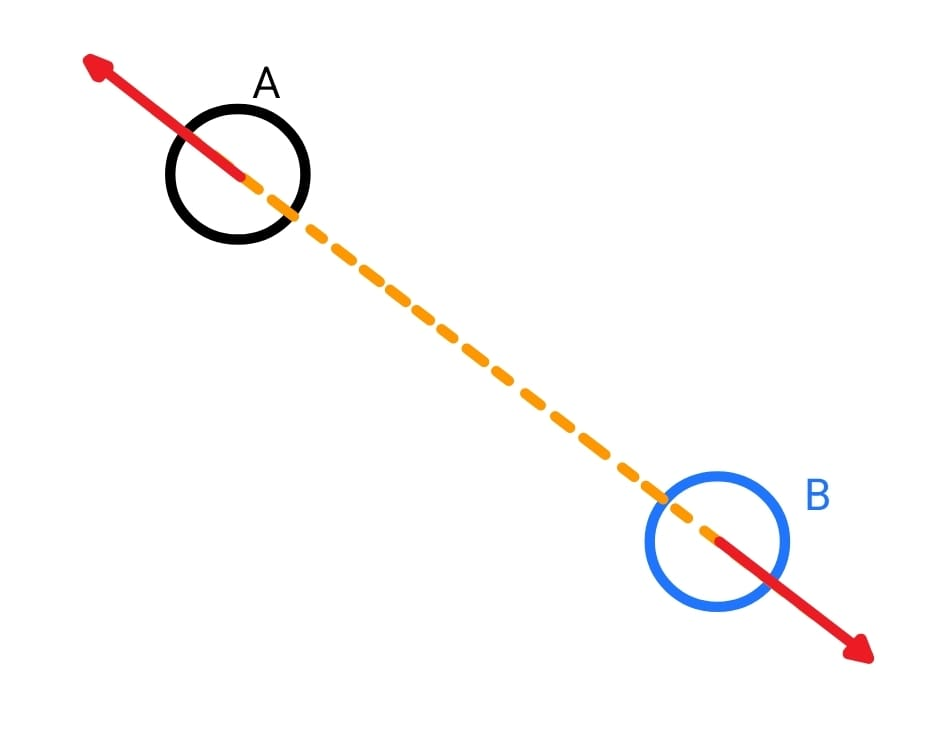
\includegraphics[width=4.5cm]{strongthirdlaw.jpeg}
			\caption{Situación del enunciado fuerte}
			\label{fig: Nthirdstrong}
		\end{figure}
	\end{marginfigure}

	\begin{marginfigure}
		\begin{figure}[H]
			\centering
			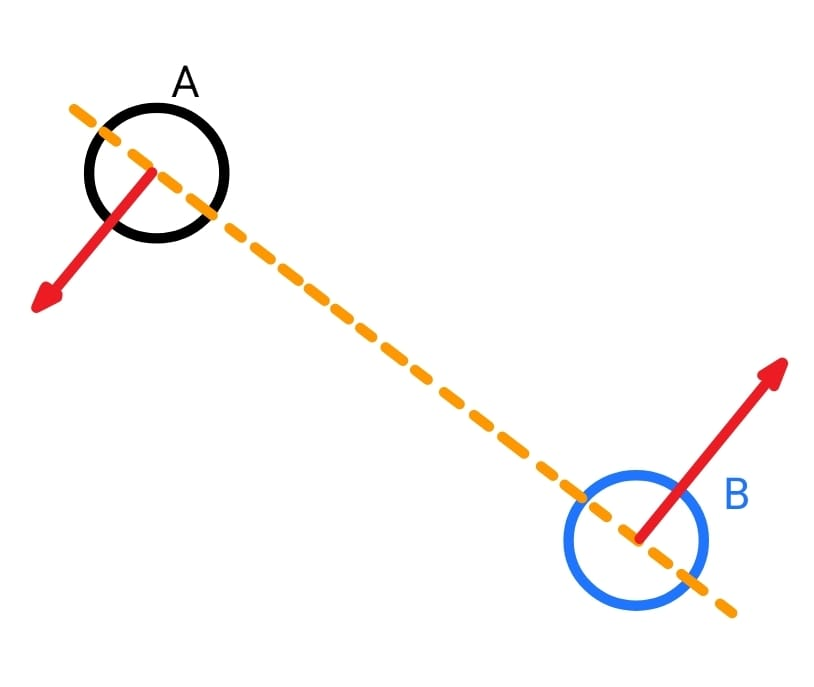
\includegraphics[width=4.5cm]{weakthirdlaw.jpeg}
			\caption{Situación del enunciado débil}
			\label{fig: Nthirdweak}
		\end{figure}
	\end{marginfigure}

	\subsection{Trabajo y Energía}

	\begin{definition}[\textbf{Trabajo}] Corresponde a la cantidad generada al tomar el producto punto de la fuerza ejercida sobre un cuerpo a lo largo de todo su desplazamiento desplazamiento desde una punto A a un punto B.
		\begin{equation}
			W = \int_{A}^{B} \vec{F} \cdot d\vec{r}
			\label{eq: work}
		\end{equation}
	\end{definition}

	\begin{definition}[\textbf{Fuerza conservativa}] Una fuerza $\vec{F}$ es conservativa si se puede escribir de la forma:
		\begin{equation}
			\vec{F} = - \vec{\nabla} V \left(\vec{r}\right)
			\label{eq: conservativeforce}
		\end{equation}
		Es decir, si el potencial que genera la fuerza depende únicamente de la posición de la partícula, será una fuerza conservativa.
	\end{definition}

	A partir de las Ecuaciones \rref{eq: NSecondlaw} y \rref{eq: work}:

	\begin{align*}
		W & = \int_{A}^{B} \vec{F} \cdot d\vec{r} \; = \; \int_{A}^{B}  \frac{d \vec{p}}{dt} \cdot d\vec{r}
	\end{align*}

	Ejerciendo el producto punto y trabajando por índices:
	\begin{align*}
		W & = \int_{A}^{B} \sum_{i=1}^{3} \frac{d p_{i}}{dt}dr_{i}
	\end{align*}

	Suponiendo que la masa es constante, la derivada temporal del momentum lineal es de la forma: $\frac{d p_{i}}{dt} = m \frac{d v_{i}}{dt}$:

	\begin{align*}
		W & =  \sum_{i=1}^{3} m \int_{A}^{B} \frac{d v_{i}}{dt}dr_{i} =  \sum_{i=1}^{3} m \int_{A}^{B} \frac{d v_{i}}{dt}dr_{i} \frac{dt}{dt}\\ 
		& = \sum_{i=1}^{3} m \int_{A}^{B} d v_{i} \underbrace{\frac{d r_{i}}{dt}}_{= \: v_{i}} \cancelto{1}{\frac{dt}{dt}}\\
		& = \sum_{i=1}^{3} m \int_{A}^{B}  v_{i} d v_{i} =  \sum_{i=1}^{3} m \int_{A}^{B} \frac{1}{2} d \left(v_{i}^{2}\right)\\
		& = \left . \sum_{i=1}^{3} \frac{1}{2} m v_{i}^{2} \right|_{A} ^{B} = \sum_{i=1}^{3} \frac{1}{2} m v_{iB}^{2} - \sum_{i=1}^{3} \frac{1}{2} m v_{iA}^{2}
	\end{align*}

	\begin{definition}[\textbf{Energía Cinética Traslacional}] Corresponde al trabajo necesario para comenzar a mover un cuerpo desde el reposo hasta la rapidez $v$.

		\begin{equation} 
			T =  \frac{1}{2} m \sum_{i=1}^{3} v_{i}^{2}
			\label{eq: Ttras}
		\end{equation}
	\end{definition}

	\begin{theorem}[\textbf{Trabajo - Energía Cinética}]

		\begin{equation}
			W = \Delta T
			\label{eq: workT}
		\end{equation}
		
	\end{theorem}

	Regresando a la definición \Eqref{eq: work} pero ahora tomando la fuerza que es ejercida sobre el cuerpo como una fuerza conservativa, \Eqref{eq: conservativeforce}.

	\begin{align*}
		W &= \int_{A}^{B} \vec{F} \cdot d\vec{r} =  \int_{A}^{B} - \vec{\nabla}V \cdot d\vec{r} = -V_{B} + V_{A}
	\end{align*}

	\begin{definition}[\textbf{Energía Potencial}] Corresponde a la capacidad de un cuerpo de ejercer trabajo se denomina energía potencial. Ahora se presentan algunos ejemplos de energías potenciales.

		\begin{equation}
			V = \left \{ \begin{matrix}
				mgh\\ 
				\\
				\frac{1}{2}kx^{2} \\
				\\
				\frac{-GMm}{r}\\ 
				\\
				\frac{-Kq_{1}q_{2}}{r}\\ 
				\vdots 
				\end{matrix} \right .
		\end{equation}
	\end{definition}

	\begin{theorem}[\textbf{Trabajo - Energía Potencial}]

		\begin{equation}
			W = - \Delta V
			\label{eq: workV}
		\end{equation}
		
	\end{theorem}

	\begin{definition}[\textbf{Energía de un sistema}]
		Ante la suposición de que el sistema a tratar tienen masa constante y es un sistema conservativo, la energía total es de la forma:
		\begin{equation}
			E = T + V
			\label{eq: Energy}
		\end{equation}
		
	\end{definition}

	\subsection{Análogo rotacional de las leyes de Newton}

	Ahora se presentarán algunos conceptos importantes y ecuaciones para una descripción sencilla de la mecánica de partículas en rotación. 	
	\begin{marginfigure}
		\begin{figure}[H]
			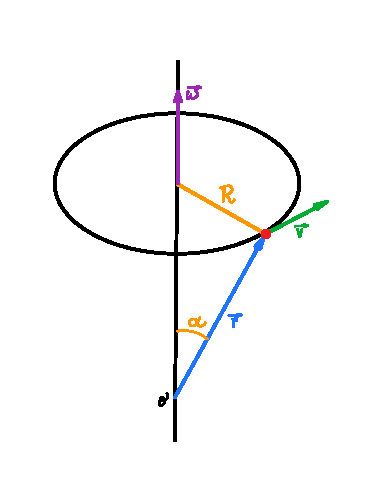
\includegraphics[width=4.8cm]{vwxr.pdf}
			\caption{Relación entre $\vec{v}$ , $\vec{\omega}$ y $\vec{r}$}
			\label{fig: vwxr}
		\end{figure}
	\end{marginfigure}
	Nuevamente se comenzará por los conceptos básicos análogos a los usados en las leyes de Newton y posteriormente se darán las leyes análogas.



	Primero deduciendo una relación entre la velocidad lineal $\vec{v}$ y la velocidad angular $\vec{\omega}$:

	$\bullet$ Se sabe que la velocidad angular es por definición
	\begin{equation}
		\vec{\omega}= \frac{d \vec{\theta}}{dt}
	\end{equation}
	respecto a un eje instantáneo de rotación. Siempre será posible establecer una velocidad angular para un cuerpo en movimiento arbitrário, ya que en cada instante el cuerpo se mueve con una trayectoría circular respecto a un eje de rotación; esto se puede observar en la \Figref{fig: vwxr}.


	Obsevando la rotación infinitesimal presente en \Figref{fig: difvwxr}, se puede concluir la siguiente relación \mn{Recuerde que antes se era bien conocida la relación $v = \omega R$ para una partícula en un movimiento circular de radio $R$ en un plano.\\ 
	\\
	En este caso, al relacionar con $\vec{r}$, se tiene: 
	\begin{center}
		$v = wr sen\left(\alpha\right)$
	\end{center}}
	

	\begin{equation*}
		\delta \vec{r} = \delta \vec{\theta} \times \vec{r}
	\end{equation*}

	Dividiente entre $\delta t$:

	\begin{equation*}
		\frac{\delta \vec{r}}{\delta t} =\frac{\delta \vec{\theta}}{\delta t}  \times \vec{r}
	\end{equation*}

	Lo cual, al considerar $\delta t \rightarrow 0$, se convierte en:

	\begin{equation*}
		\frac{d \vec{r}}{dt} = \frac{d \vec{\theta}}{dt} \times \vec{r}
	\end{equation*}

	\begin{definition}[\textbf{Relación velocida Lineal - Angular}]
		Para un cuerpo en un movimiento arbitrário se cumple lo siguiente para cada instante del movimiento.
		\begin{equation}
			\vec{v} = \vec{w} \times \vec{r}
			\label{eq: vwrelation}
		\end{equation}
		Recuerde que el eje de rotación instantáneo puede cambiar si el movimiento no es una rotación fija.
	\end{definition}


	\begin{marginfigure}
		\begin{figure}[H]
			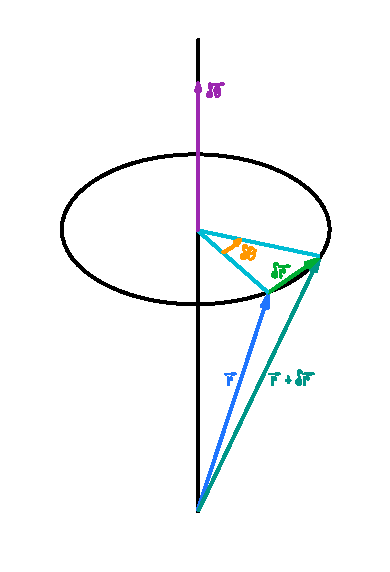
\includegraphics[width=5cm]{difvwxr.pdf}
			\caption{Relación diferencial entre $\vec{v}$ , $\vec{\omega}$ y $\vec{r}$}
			\label{fig: difvwxr}
		\end{figure}
	\end{marginfigure}

	\begin{definition}[\textbf{Torque}]
		El torque es el análogo de la fuerza para las rotaciones. Por lo que el torque corresponde a una interacción del sistema con su entorno que es capaz de generar un cambio en el estado \textit{rotacional} del sistema, dicha interacción es mediada por la presencia de una o más fuerzas y se define como:
		\begin{equation}
			\vec{N}_{\mathcal{O}} = \vec{r} \times \vec{F}
			\label{eq: torque}
		\end{equation}
		Como tal, el torque depende del origen que se este utilizando, debido a su dependencia con el vector posición $\vec{r}$. Al torque es común llamarlo en algunos campos como: torca, momento de fuerza o simplemente momento.
	\end{definition}

	\begin{definition}[\textbf{Momentum Angular}]
		Corresponde al análogo angular del momentum lineal. Es una cantidad vectorial que para el caso de partículas se define como:
		\begin{equation}
			\vec{L}_{\mathcal{O}} = \vec{r} \times \vec{p} = m\; \vec{r} \times \vec{v} = m\; \vec{r} \times \left(\vec{\omega} \times \vec{r} \right) \textup{\textcolor{blue}{\mn{$\vec{A} \times \left(\vec{B} \times \vec{C}\right) = \vec{B} \left(\vec{A}\cdot\vec{B}\right) - \vec{C}\left(\vec{A} \cdot \vec{B}\right)$}}} = m \left[\vec{r}\;^{2} \vec{\omega} - \vec{r} \left(\vec{r} \cdot \vec{\omega}\right)\right]
			\label{eq: momentumA}
		\end{equation}

		De forma similar al torque, el momentum angular depende del origen desde el que se decida medir.\\

		En la amplia gama de casos en que se trabaja con partículas, se podrá reconocer que el producto $\vec{r} \cdot \vec{\omega} = 0$ y los vectores $\vec{r}$ y $\vec{\omega}$ apuntan en una única dirección, por lo que el momentum angular tomará la siguiente forma:

		\begin{equation}
			L_{\mathcal{O}q} = m  r^{2} \omega_{q}
		\end{equation}
	\end{definition}

	\marginnote{La \textbf{masa} \textit{inercial} y los \textbf{ momentos de inercia}  están intimamente relacionados, ambos son medidas de que tan difícil es mover un cuerpo de cierta forma.}

	\begin{definition}[\textbf{Momentos de Inercia}]
		La inercia es el análogo rotacional de la masa y corresponde a una medida que indica que tan difícil es girar un cuerpo respecto a cada eje (A mayor inercia más complicado es girar el objeto). Girando un cuerpo es posible concluir que se pueden generar rotaciones respecto a 3 ejes y por lo tanto \textbf{existen 3 momentos de inercia}, los cuales no necesariamente serán iguales, esto dependerá de la distribución de la masa respecto a cada eje.

		En el caso de partículas puntuales, la inercia se define como:
		
		\begin{equation}
			I_{q}^{\mathcal{O}} = \sum_{i} m_{i} r^{2}_{i}
			\label{eq: easyinercia}
		\end{equation}

		Donde $r_{i}$ corresponde a la distancia que hay entre el eje de rotación y la masa puntual.

	\end{definition}

	\marginnote{El termino \textit{inercial} es para hacer una distinción entre la \textbf{masa inercial} (La masa dada por la aceleración de un cuerpo al estar bajo el efecto de una fuerza) y la \textbf{masa gravitacional} (La masa determinada por las fuerzas gravitacionales entre el cuerpo de interés y otros cuerpos), a pesar de que ambas cantidades \textbf{son iguales} por el princiopio de equivalencia. }

	\begin{definition}[\textbf{Primera Ley de Newton análoga rotacional}]
		De forma similar a la Primera Ley de Newton, este princiopio análogo estable que un cuerpo en un estado rotacional de equilibrio tenderá a mantener dicho estado hasta que un torque neto diferente de cero lo perturbe.
		\begin{equation}
			\sum \vec{N}_{\mathcal{O}} = 0
			\label{eq: Nfirstlawrot}
		\end{equation}
		
	\end{definition}

	\begin{definition}[\textbf{Segunda Ley de Newton análoga rotacional}]
		\begin{equation}
			\sum \vec{N}_{\mathcal{O}} = \frac{d \vec{L}_{\mathcal{O}}}{dt} = \dot{\vec{L}}_{\mathcal{O}}
			\label{eq: NSecondlawrot}
		\end{equation}

		Manteniendo la inercia constante, la ecuación se escribe de la forma:
		\begin{equation}
			\sum N_{q} = I_{q} \alpha_{q}
		\end{equation}
		Donde el subíndice denota el eje respecto al cual se está realizando la suma de torques.
	\end{definition}

	\newpage
	\begin{definition}[\textbf{Tercera Ley de Newton análoga rotacional}] 
		Este principio se enuncia de forma análoga a la Tercera Ley de Newton original bajo la salvedad de que en vez de trabajar con fuerzas, este trabaja con torques.

		\begin{equation}
			\vec{N}_{AB} = - \vec{N}_{BA}
			\label{eq: NThirdlawrot}
		\end{equation}
		
	\end{definition}

	\begin{definition}[\textbf{Energía Cinética Rotacional}]
		Corresponde al trabajo necesario para hacer rotar un cuerpo desde el reposo hasta la rapidez angular $\omega$.
		\begin{equation}
			T_{rot} = \frac{1}{2}I_{q}\omega^{2}
			\label{eq: Trot}
		\end{equation}
		La forma de obtener esta expresión es similar al procedimiento que se realizó con la energía cinética traslacional.
	\end{definition}

	\subsection{Teoremas de Conservación}

	A continuación se van a enunciar los teoremas de conservación bajo la suposición de masa constante y que el sistema a tratar no posee fuerzas disipativas.


	\begin{theorem}[\textbf{Conservación de la Energía}]
		Una vez ya conocida la expresión para la energía del sistema \Eqref{eq: Energy}, basta con derivarla con respecto al tiempo para determinar que restricciones se plantean para la conservación de dicha cantidad:

		\begin{align*}
			E = T + V \Rightarrow \frac{dE}{dt} & = \frac{dT}{dt} + \frac{dV}{dt} \; \textup{; A partir de \Eqref{eq: Ttras} y suponiendo $V = V(\vec{r}, t)$}\\
												& = \frac{d}{dt} \left(\frac{1}{2} m \dot{\vec{r}}\:^{2}\right) + \overbrace{\sum_{i=1}^{3} \frac{\partial V}{\partial x_{i}} \frac{d x_{i}}{d t}}^{= \vec{\nabla}V \cdot \dot{\vec{r}}} + \cancelto{0}{\frac{\partial V}{\partial t}} \; \; ; \left .\begin{matrix}
													\textup{Sistema}\\ 
													\textup{conservativo}
													\end{matrix} \right . \Rightarrow V = V(\vec{r}) \\
												& = \frac{1}{2} m \left(\ddot{\vec{r}} \cdot \dot{\vec{r}} + \dot{\vec{r}} \cdot \ddot{\vec{r}}\right) + \vec{\nabla} V \dot{\vec{r}} 
												= m \ddot{\vec{r}} \cdot \dot{\vec{r}} + \vec{\nabla} V \dot{\vec{r}}
												= \left[m \ddot{\vec{r}} +   \vec{\nabla} V \right] \dot{\vec{r}}\\
												& = \left[\vec{F} + \vec{\nabla} V \right] \cdot \dot{\vec{r}}\\
		\end{align*}

		Para que la energía se conserve se cumple:

		\begin{align*}
			\Rightarrow \frac{dE}{dt} = \left[\vec{F} + \vec{\nabla} V \right] \cdot \dot{\vec{r}} = 0
			&\Rightarrow \vec{F} + \vec{\nabla} V = 0\\
			& \Rightarrow \vec{F} = - \vec{\nabla} V 
		\end{align*}

		\begin{equation}
			\therefore \frac{dE}{dt} = 0 \Rightarrow  \vec{F} = - \vec{\nabla} V
			\label{eq: Econs}
		\end{equation}
		
	\end{theorem}

	\begin{theorem}[\textbf{Conservación de Momentum Lineal}]
		Conociendo ya la expresión de la \Eqref{eq: momentuml}, se derivará con respecto al tiempo para determinar las condiciones en que se conserva dicha cantidad:

		\begin{align*}
			\vec{p} = m \dot{\vec{r}} \Rightarrow \frac{d\vec{p}}{dt} &= \cancelto{0}{\frac{dm}{dt}} \dot{\vec{r}} + m \ddot{\vec{r}}\\ 
																	& = m \ddot{\vec{r}} = \vec{F}
		\end{align*}

		Para que el momentum lineal se conserve se cumple: 

		\begin{align*}
			\Rightarrow \frac{d\vec{p}}{dt} = m \ddot{\vec{r}} = \vec{F} = \vec{0}
		\end{align*}


		\begin{equation}
			\therefore \frac{d\vec{p}}{dt} = 0 \Rightarrow \vec{F} = \vec{0}
			\label{eq: momentumlcons}
		\end{equation}
		
	\end{theorem}

	\begin{theorem}[\textbf{Conservación de Momentum de Angular}]
		A partir de la expresión de la \Eqref{eq: momentumA} y derivandola respecto al tiempo:
		\begin{align*}
			\vec{L}_{\mathcal{O}} = \vec{r} \times \vec{p} \Rightarrow \frac{d \vec{L}_{\mathcal{O}}}{dt} & = \overbrace{\dot{\vec{r}} \times \vec{p}}^{\dot{\vec{r}} \: \parallel \: \vec{p} } + \vec{r} \times \dot{\vec{p}} \\ 
			& = \vec{r} \times \dot{\vec{p}} \; \; \; \textup{; Por la \Eqref{eq: NSecondlaw}} \\ 
			& =  \vec{r} \times \vec{F} \; \; \; \textup{; Por la \Eqref{eq: torque}} \\
			& = \vec{N}_{\mathcal{O}}
		\end{align*}
		Para que se conserve el momentum angular se debe cumplir:

		\begin{equation*}
			\Rightarrow \frac{d \vec{L}_{\mathcal{O}}}{dt} =  \vec{r} \times \vec{F} = \vec{N}_{\mathcal{O}} = \vec{0}
		\end{equation*}

		\begin{equation}
			\therefore \frac{d \vec{L}_{\mathcal{O}}}{dt} = 0 \Rightarrow  \vec{N}_{\mathcal{O}} = \vec{0}
			\label{eq: momentumAcons}
		\end{equation}
	\end{theorem}

	\newpage
	\subsection{Complementos de la conservación de la energía}

	\begin{definition}[\textbf{Condiciones de estabilidad}]
		
		Al conservarse la energía en un sistema, es posible encontrarse con que la partícula de interés se encuentra en un punto de equilibrio de algún tipo (Estables u Inestables), alrededor de estos puntos es posible obtener mucha información acerca del comportamiento del sistema. Las siguientes son las condiciones para determinar que es un punto de equilibrio y clasificarlo.

		\begin{itemize}
			\item \textbf{Punto de equilibrio: } Se define como un punto en algun potencial que cumple con: \\ 
				\begin{equation}
				\left .  \vec{\nabla }V \right|_{\vec{r} \: = \: \vec{r}_{eq}} = 0
				\end{equation}
			\begin{itemize}
				\item Punto de Equilibrio \textcolor{red}{Estable}: De colocar una partícula en reposo en este punto y sin la aparición de fuerzas a su alrededor, la partícula permanecerá en equilibrio en dicho punto por siempre. Ahora, si esta es colocada en reposo en los alrededores de este punto o desde el punto de equilibrio se le ejerce una fuerza que la obligue a moverse, la partícula comenzará un movimiento en dirección a este punto y se moverá perpetuamente a su alrededor siempre que $E =$ constante. La forma de determinar los puntos estables: \\ 
				\begin{equation}
					\left .  \vec{\nabla }^{2}V \right|_{\vec{r} \: = \: \vec{r}_{eq}} > 0
					\label{eq: puntoestable}
				\end{equation}
				\item Punto de Equilibrio \textcolor{red}{Inestable}: De forma similar al anterior, si se coloca una partícula en reposo en este punto y sin la aparición de fuerzas a su alrededor, la partícula permanecerá en equilibrio en dicho punto por siempre. No obstante, de aparecer algún tipo de fuerza o colocarla en los alrededores del punto de equilibrio inestable, la partícula se encontrará en un movimiento unicamente limitado por la cantidad de energía del sistema y es posible que nunca vuelva a pasar por dicho punto. La forma de encontrar los puntos inestables: \\  
				\begin{equation}
					\left .  \vec{\nabla }^{2}V \right|_{\vec{r} \: = \: \vec{r}_{eq}} < 0
					\label{eq: puntoinestable}
				\end{equation}
				\item Punto \textcolor{red}{No concluyente}:  				
				\begin{equation}
					\left .  \vec{\nabla }^{2}V \right|_{\vec{r} \: = \: \vec{r}_{eq}} = 0
					\label{eq: puntonoconcluyente}
				\end{equation}
				\\Es necesario comprobar derivadas de orden superior bajo los mismos criterios para determinar estabilidad u inestabilidad de la posición de equilibrio. De obtenerse  $\left .  \vec{\nabla }^{3}V \right|_{\vec{r} \: = \: \vec{r}_{eq}} = 0$, es necesario continar con orden 4 en la derivación, comprobar criterios y, de ser necesario, repetir los pasos en derivaciones superiores.
			\end{itemize}
		\end{itemize}
	\end{definition}

	A continuación se muestra un ejemplo de como se aplican estos conceptos en un caso unidimensional.
	\begin{figure}[H]
		\centering
		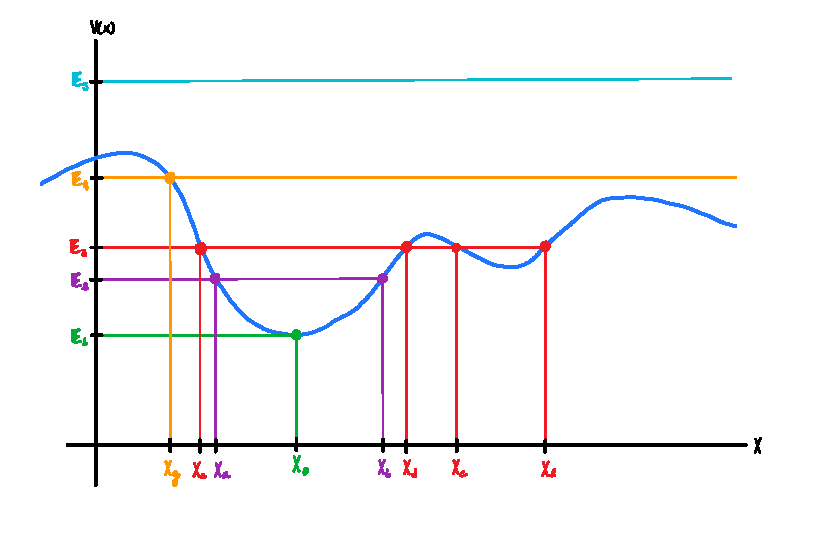
\includegraphics[width=15cm]{puntosequilibrio.pdf}
		\caption{Ejemplo en una dimensión de las condiciones de estabilidad. \\ La línea azul corresponde a la energía potencial que siente la partícula en cada punto. Se colocan un total de 5 energías totales para el sistema cada una determinada por un color para mayor facilidad. Junto a esto, cada intersección que tienen las rectas de energía con la curva de potencial posee un punto y también su respectiva ubicación en el eje X acorde al color de la energía total.}
		\label{fig: puntosequilibrio}
	\end{figure}

	Al observar la \Figref{fig: puntosequilibrio}, se determina lo siguente:

	\begin{itemize}
		\item $x = x_{0}$ corresponde a un punto de equilibrio estable.
		\item Si se coloca una partícula en $x = x_{0}$ en energía \textcolor{green}{$E_{1}$} , esta permancerá en reposo.
		\item Para la energía \textcolor{violet}{$E_{2}$} , la partícula se moverá de forma periódica en $x_{a} < x < x_{b}$.
		\item Para la energía \textcolor{red}{$E_{3}$}, la partícula se moverá de forma periódica en $x_{c} < x < x_{d}$ ó $x_{e} < x < x_{f}$. Esto es excluyente cabe destacar, la partícula se movera en uno o en el otro foso.
		\item Hay un punto de equilibrio inestable entre los puntos $x_{d}$ y $x_{e}$, al igual que entre $x = 0$ y $x_{g}$.
		\item Para la energía \textcolor{orange}{$E_{4}$}, la partícula se moverá de forma periódica en $x_{g} < x < +\infty $. La partícula va a $+\infty$, vuelve a $x_{g}$ y regresa a $+\infty$, completando un ciclo.
		\item Para la energía \textcolor{cyan}{$E_{5}$}, el movimiento no está limitado por la energía potencial que siente la partícula. Esta se puede mover libremente pero su velocidad va a depender de la posición en la que se encuentre.
	\end{itemize}


	\subsection{Problemas resueltos}

	\includepdf[pages={27-53},templatesize = {8 in}{8.5 in} ]{AMeca.pdf}
	

	\section{Sistemas de partículas}
	\label{sec: sisparticulas}

	\subsection{Suposiciones iniciales}

    Para trabajar con sistemas de partículas $N$ es necesario realizar ciertas suposiciones respecto a las fuerzas internas al sistema de partículas.

    \begin{itemize}
        \item Para dos partículas $\alpha$ y $\beta$ se cumple: $\vec{f}_{\alpha \beta} = - \vec{f}_{\beta \alpha}$.
        \item Los vectores fuerza están sobre la línea que une a ambas partículas.
    \end{itemize}
    Estas dos suposiciones se pueden resumir al aceptar trabajar con el \textbf{Enunciado Fuerte de la Tercera Ley de Newton}  (\Figref{fig: Nthirdstrong}). De acuerdo a esto, se procederá a construir las expresiones para sistemas de partículas para los conceptos conocidos en la sección anterior y a introducir algunos conceptos nuevos.


    \begin{marginfigure}
        \begin{figure}[H]
            \centering
            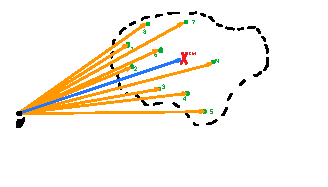
\includegraphics[width=6.5cm]{cm.pdf}
            \caption{Un sistema arbitrário con su respectivo centro de masa}
            \label{fig: centrodemasa}
        \end{figure}
    \end{marginfigure}

    \begin{definition}[\textbf{Centro de masa}]
        Corresponde a un punto del espacio en que se encuentra el sistema de partículas (discreto o continuo) en el cual es posible colapsar toda la masa del sistema, de modo que una fuerza arbitrária que interactue con alguna partícula del sistema se podrá transportar a dicho punto para conocer la mecánica del sistema (\Figref{fig: centrodemasa}). El centro de masa se define a partir de un promedio ponderado de toda la masa del sistema visto a continuación:

        \begin{align}
            \vec{R} = \frac{1}{M} \sum_{\alpha =1}^{N} m_{\alpha} \vec{r}_{\alpha} \; \; \rightarrow  & \; \; \vec{R} = \frac{1}{M} \int_{M} \vec{r} dm \\ 
            M = \sum_{\alpha = 1}^{N} m_{\alpha} \; \; \rightarrow  & \; \; M =  \int_{M}  \rho dV
        \end{align}
        
    \end{definition}

	\subsection{Definición de la mecánica de sistemas de partículas}

	Para definir la expresión del momentum lineal de un sistema de partículas hay que construirla a partir del conocimiento de la sección anterior. A partir de esto, se definen las siguientes cantidades para la partícula $\alpha$ del sistema:

	\begin{itemize}
		\item Fuerza neta externa al sistema sobre $\alpha$: $\vec{F}_{\alpha}^{e}$ 
		\item Fuerza neta interna al sistema sobre $\alpha$: $\vec{f}_{\alpha}= \sum_{\left .\begin{matrix} \beta = 1\\ \alpha \neq \beta \end{matrix}\right .}^{N}\vec{f}_{\alpha \beta}$ 
	\end{itemize}

		Entonces la fuerza neta que percibe la partícula $\alpha$ es:
		\begin{equation*}
			\vec{F}_{\alpha} = \vec{F}_{\alpha}^{e} + \vec{f}_{\alpha}
		\end{equation*}
		De acuerdo a la Segunda Ley de Newton \Eqref{eq: NSecondlaw}:

		\begin{align*}
			& \dot{\vec{p}}_{\alpha} = \vec{F}_{\alpha} = m_{\alpha}\ddot{\vec{r}}_{\alpha} \\ 
			\Rightarrow \; & m_{\alpha}\ddot{\vec{r}}_{\alpha} = \vec{F}_{\alpha}^{e} + \vec{f}_{\alpha}
		\end{align*}

		Hasta este momento se ha estado trabajando unicamente con la partícula $\alpha$, pero si ahora sumamos la expresión anterior para todas las partículas, se obtiene:

		\begin{align*}
			\Rightarrow \; \sum_{\alpha  = 1}^{N} \left[m_{\alpha} \vec{r}_{\alpha}\right] & = \sum_{\alpha = 1}^{N} \vec{F}_{\alpha}^{e} + \sum_{\alpha = 1}^{N} \vec{f}_{\alpha} \\ 
			& = \sum_{\alpha = 1}^{N} \vec{F}_{\alpha}^{e} + \sum_{\alpha = 1}^{N} \sum_{\left .\begin{matrix} \beta = 1\\ \alpha \neq \beta \end{matrix}\right .}^{N}\vec{f}_{\alpha \beta} \\ 
			& =  \sum_{\alpha = 1}^{N} \vec{F}_{\alpha}^{e} + \sum_{\left .\begin{matrix} \alpha \: , \: \beta = 1\\ \alpha \neq \beta \end{matrix}\right .}^{N}\vec{f}_{\alpha \beta} \\ 
			\Rightarrow \underbrace{\sum_{\alpha  = 1}^{N} \frac{d^{2}}{dt^{2}} \left[m_{\alpha} \vec{r}_{\alpha}\right]}_{M \vec{r}_{CM}} & = \underbrace{ \sum_{\alpha = 1}^{N} \vec{F}_{\alpha}^{e}}_{\vec{F}} \; \; + \cancelto{0}{\sum_{\left . \begin{matrix} \alpha \: , \: \beta = 1\\ \alpha \neq \beta \end{matrix} \right .}^{N}\vec{f}_{\alpha \beta}}
		\end{align*} 

		De esta última expresión se obtiene \mn{El término \begin{equation*} \sum_{\left . \begin{matrix} \alpha \: , \: \beta = 1\\ \alpha \neq \beta \end{matrix} \right .}^{N}\vec{f}_{\alpha \beta} \end{equation*} \\ se hace cero porque se tiene:  \begin{equation*} \sum_{\alpha < \beta = 1}^{N} \vec{f}_{\alpha \beta} + \vec{f}_{\beta \alpha}\end{equation*} y es evidente que estas son fuerzas contrarias de igual magnitud debido a la \textbf{Tercera Ley de Newton}, por lo que el resultado de su suma es cero.}

		\begin{align*}
			\vec{F} = \dot{\vec{P}} \; \; \; \; \; \; &y \; \; \; \; \; \; \vec{P} = \sum_{\alpha = 1}^{N} m_{\alpha} \dot{\vec{r}}_{\alpha} = M\dot{\vec{R}}
		\end{align*}

    \begin{definition}[\textbf{Momentum Lineal y Segunda Ley de Newton para un Sistema}] 
		La expresión para el momentum lineal de un sistema de partículas:
		\begin{equation}
			\vec{P} = M\dot{\vec{R}}
			\label{eq: sismomentuml}
		\end{equation}

		y la expresión de la Segunda Ley de Newton para el caso de un sistema de partículas en el caso traslacional:

		\begin{equation}
			\vec{F} = \dot{\vec{P}} = M \ddot{\vec{R}}
			\label{eq: sisNSecondlaw}
		\end{equation}
    \end{definition}

	\newpage

	Ahora se resolverá un procedimiento similar para hallar una expresión para el momentum angular de un sistema de partículas respecto a un punto $\mathcal{O}$:

	El momentum angular de una partícula $\alpha$ desde el punto $\mathcal{O}$ (Ver \Figref{fig: sismangular1}) es: 

	\begin{equation*}
		\vec{L}_{\alpha}^{\mathcal{O}} = \vec{r}_{\alpha} \times \vec{p}_{\alpha}
	\end{equation*}

	\begin{marginfigure}
		\begin{figure}[H]
			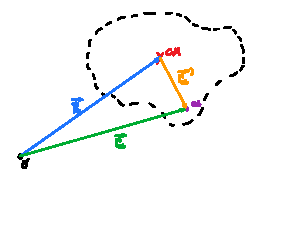
\includegraphics[width=7cm]{sismangular1.pdf}
			\caption{Posición de la partícula $\alpha$ y el centro de masa de un sistema respecto a $\mathcal{O}$}
			\label{fig: sismangular1}
		\end{figure}
	\end{marginfigure}

	Si se realiza la suma de todos lo momentums angulares individuales, esto da a como resultado el momentum angular del sistema:

	\begin{align*}
		\vec{L}^{\mathcal{O}} &= \sum_{\alpha = 1}^{N} \vec{r}_{\alpha} \times \vec{p}_{\alpha} \\ 
							& = \sum_{\alpha = 1}^{N} \vec{r}_{\alpha} \times \left(m_{\alpha} \vec{v}_{\alpha} \right) \\ 
							& = \sum_{\alpha = 1}^{N} \left(\vec{R} + {\vec{r}}\,'_{\alpha} \right) \times \left[m_{\alpha} \left(\dot{\vec{R}} + {\dot{\vec{r}}}\,'_{\alpha} \right) \right] \\ 
							& = \sum_{\alpha =1}^{N} m_{\alpha} \left({\vec{r}}\,'_{\alpha} \times {\dot{\vec{r}}}\,'_{\alpha} + {\vec{r}}\,'_{\alpha} \times \dot{\vec{R}} + \vec{R} \times {\dot{\vec{r}}}\,'_{\alpha} + \vec{R} \times \dot{\vec{R}} \right) \\ 
							& =  \sum_{\alpha =1}^{N} m_{\alpha} {\vec{r}}\,'_{\alpha} \times {\dot{\vec{r}}}\,'_{\alpha} + \textcolor{blue}{\sum_{\alpha =1}^{N} m_{\alpha} {\vec{r}}\,'_{\alpha} \times \dot{\vec{R}} + \sum_{\alpha =1}^{N} m_{\alpha} \vec{R} \times {\dot{\vec{r}}}\,'_{\alpha}} + \sum_{\alpha =1}^{N} m_{\alpha}  \vec{R} \times \dot{\vec{R}}
	\end{align*}


	\begin{marginfigure}
		\begin{figure}[H]
			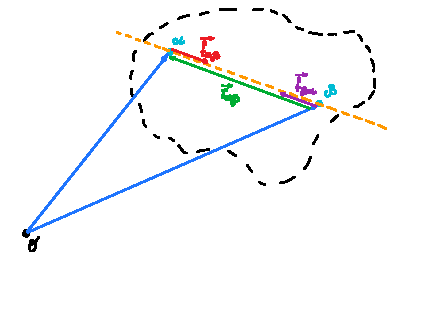
\includegraphics[width=7cm]{sismangular2.pdf}
			\caption{Interacción y posiciones de las partículas $\alpha$ y $\beta$ de un sistema respecto a $\mathcal{O}$ }
			\label{fig: sismangular2}
		\end{figure}
	\end{marginfigure}

	Trabajando por un momento con los terminos en azul:

	\begin{align*}
		& \sum_{\alpha =1}^{N} m_{\alpha} {\vec{r}}\,'_{\alpha} \times \dot{\vec{R}} + \sum_{\alpha =1}^{N} m_{\alpha} \vec{R} \times {\dot{\vec{r}}}\,'_{\alpha} \\ 
		& = \left( \sum_{\alpha =1}^{N} m_{\alpha} {\vec{r}}\,'_{\alpha} \right) \times \dot{\vec{R}} + \vec{R} \times \frac{d}{dt} \left( \sum_{\alpha =1}^{N} m_{\alpha} {\vec{r}}\,'_{\alpha} \right) \\ 
		& = \left( \sum_{\alpha =1}^{N} m_{\alpha} {\vec{r}}\,'_{\alpha} \right) \times \left( \dot{\vec{R}}  - \vec{R}\right) \\ 
		& = \left[ \sum_{\alpha =1}^{N} m_{\alpha} \left(\vec{r}_{\alpha} - \vec{R} \right) \right] \times \left( \dot{\vec{R}}  - \vec{R}\right) \\ 
		& = \left[ \sum_{\alpha =1}^{N} m_{\alpha} \vec{r}_{\alpha} -\left( \sum_{\alpha =1}^{N} m_{\alpha} \right) \vec{R} \right] \times \left( \dot{\vec{R}}  - \vec{R}\right) \\ 
		& = \cancelto{0}{\left[M\vec{R}-M\vec{R}\right]} \times \left( \dot{\vec{R}}  - \vec{R}\right) \\ 
		& = 0
	\end{align*}

	Quedando claro que ambos terminos en azul son cero por como se definición del centro de masa\mn{La posición del centro de masa respecto al centro de masa siempre será cero.}, se continuará con la expresión trasanterior:

	\begin{align*}
		\vec{L}^{\mathcal{O}} &= \sum_{\alpha =1}^{N} m_{\alpha} {\vec{r}}\,'_{\alpha} \times {\dot{\vec{r}}}\,'_{\alpha} + \cancelto{0}{\sum_{\alpha =1}^{N} m_{\alpha} {\vec{r}}\,'_{\alpha} \times \dot{\vec{R}} + \sum_{\alpha =1}^{N} m_{\alpha} \vec{R} \times {\dot{\vec{r}}}\,'_{\alpha}} + \sum_{\alpha =1}^{N} m_{\alpha}  \vec{R} \times \dot{\vec{R}} \\ 
		& = \sum_{\alpha =1}^{N} m_{\alpha} {\vec{r}}\,'_{\alpha} \times {\dot{\vec{r}}}\,'_{\alpha} + \sum_{\alpha =1}^{N} m_{\alpha}  \vec{R} \times \dot{\vec{R}} \\ 
		& = \underbrace{\sum_{\alpha =1}^{N} {\vec{r}}\,'_{\alpha} \times {\dot{\vec{p}}}\,'_{\alpha}}_{\textup{Momentum Angular alrededor del CM}} + \underbrace{M \vec{R} \times \dot{\vec{R}}}_{\textup{Momentum Angular del CM alrededor a $\mathcal{O}$}}
	\end{align*}

	Ahora, buscando la expresión para la derivada respecto al tiempo del momentum angular del sistema. Para esto hay que comenzar de forma similar, analizar desde una unica partícula puntual que forme parte del sistema de partículas:

	\begin{equation*}
		\dot{\vec{L}}_{\alpha}^{\mathcal{O}} = \vec{r}_{\alpha} \times \dot{\vec{p}}_{\alpha} = \vec{r}_{\alpha} \times \left(\vec{F}_{\alpha}^{e} + \sum_{\left . \begin{matrix} \beta = 1\\ \alpha \neq \beta \end{matrix} \right .}^{N} \vec{f}_{\alpha \beta}\right)
	\end{equation*}

	Sumando para todas las partículas \mn{Aquí se encuentra una situación similar a la que se tuvo con el momentum lineal, el termino que se canceló, es cero por lo siguiente: \\ La expresión:  \begin{equation*} \sum_{\left .\begin{matrix} \alpha\, , \, \beta = 1\\ \alpha \neq \beta \end{matrix}\right .}^{N} \vec{r}_{\alpha} \times \vec{f}_{\alpha \beta} \end{equation*} es posible reescribirla como: \begin{equation*} \sum_{\alpha < \beta =1}^{N} \left( \vec{r}_{\alpha} \times \vec{f}_{\alpha \beta} + \vec{r}_{\beta} \times \vec{f}_{\beta \alpha} \right) \end{equation*} y aquí tomando que se cumple el \textbf{Enunciado Fuerte} de la Tercera Ley de Newton \Eqref{eq: NThirdlaw} y la siguiente definición (Ver \Figref{fig: sismangular2}): \begin{equation*} \vec{r}_{\alpha \beta} = \vec{r}_{\alpha} -\vec{r}_{\beta} \end{equation*} La expresión de interés se convierte en: \begin{align*} &\sum_{\alpha < \beta =1}^{N} \left( \vec{r}_{\alpha} \times \vec{f}_{\alpha \beta} - \vec{r}_{\beta} \times \vec{f}_{\alpha \beta} \right) \\ & = \sum_{\alpha < \beta =1}^{N} \left( \vec{r}_{\alpha}  - \vec{r}_{\beta}  \right) \times \vec{f}_{\alpha \beta} \\ & = \sum_{\alpha < \beta =1}^{N}  \underbrace{\vec{r}_{\alpha \beta} \times \vec{f}_{\alpha \beta}}_{\vec{r}_{\alpha \beta} \parallel \vec{f}_{\alpha \beta}}\\ & = 0 \end{align*}}:

	\begin{align*}
		\dot{\vec{L}}_{\mathcal{O}} = \sum_{\alpha = 1}^{N} \vec{r}_{\alpha} \times \vec{F}_{\alpha}^{e} + \cancelto{0}{\sum_{\left .\begin{matrix} \alpha\, , \, \beta = 1\\ \alpha \neq \beta \end{matrix}\right .}^{N} \vec{r}_{\alpha} \times \vec{f}_{\alpha \beta}}
	\end{align*}

	De esta última expresión se obtiene:

	\begin{align*}
		& \dot{\vec{L}}_{\mathcal{O}} = \sum_{\alpha = 1}^{N} \vec{r}_{\alpha} \times \vec{F}_{\alpha}^{e} = \sum_{\alpha=1}^{N} \vec{N}_{\alpha} ^{e} \\ 
		\Rightarrow \; & \dot{\vec{L}}_{\mathcal{O}} = \vec{N}
	\end{align*}

	\begin{definition}[\textbf{Momentum Angular y Análogo Rotacional de la Segunda Ley de Newton para Sistemas}]
		La expresión del momentum angular para un sistema de partículas
		\begin{equation}
			\vec{L}^{\mathcal{O}} = \underbrace{\sum_{\alpha =1}^{N} {\vec{r}}\,'_{\alpha} \times {\dot{\vec{p}}}\,'_{\alpha}}_{\textup{Momentum Angular alrededor del CM}} + \underbrace{M \vec{R} \times \dot{\vec{R}}}_{\textup{Momentum Angular del CM alrededor a $\mathcal{O}$}}
			\label{eq: sismomentumA}
		\end{equation}
		La expresión del análogo rotacional para un sistema de partículas de la Segunda Ley de Newton:
		\begin{equation}
			\vec{N} = \dot{\vec{L}}_{\mathcal{O}}
			\label{eq: sisNSecondlawrot}
		\end{equation}
	\end{definition}

	El siguiente es el resultado ya conocido del Teorema de Ejes paralelos, el cual puede ser útil para resolver problemas concernientes a este tema.

	\begin{theorem}[\textbf{Teorema de Ejes paralelos}]
		\begin{equation}
			I_{{q}'}= I_{q}^{cm} + Md^{2}
		\end{equation}

		La demostración de este teorema tal y como se encuentra escrito aquí se le dejará al lector y se recomienda verlo como una simplificación del teorema de ejes paralelos real que se desarrollará más adelante.
	\end{theorem}

	Ahora hay que estudiar la forma de la energía cinética para un sistema de partículas. Para esto se va a empezar la deducción desde el trabajo de mover la partícula $\alpha$ de un punto a otro para la posterior definición de la energía cinética del sistema: 

	\begin{equation*}
		W_{\alpha}^{AB} = \int_{A}^{B} \vec{F}_{\alpha} \cdot d\vec{r}_{\alpha}
	\end{equation*}
	Sumando para todo el sistema: 
	\begin{equation*}
		W_{AB} = \sum_{\alpha = 1}^{N} \int_{A}^{B} \vec{F}_{\alpha} \cdot d\vec{r}_{\alpha} = \sum_{\alpha = 1}^{N} \int_{A}^{B} d\left(\frac{1}{2} m_{\alpha}v_{\alpha}^{2}\right)
	\end{equation*}
	Entonces, en una primera instancia se puede definir la energía cinética del sistema como:

	\begin{equation*}
		T = \sum_{\alpha =1}^{N} T_{\alpha} = \sum_{\alpha =1}^{N} \frac{1}{2} m_{\alpha}v_{\alpha}^{2}	
	\end{equation*}

	Pero se está buscando una expresión que tome en cuenta el centro de masa, entonces hay que continuar trabajando con este último resultado. Recordando de la \Figref{fig: sismangular1} lo siguiente: $\vec{r}_{\alpha} = \vec{R} + {\vec{r}}\,'_{\alpha}$. De aquí se obtine:

	\begin{equation*}
		\vec{r}_{\alpha} = \vec{R} + {\vec{r}}\,'_{\alpha} \Rightarrow \; \dot{\vec{r}}_{\alpha} = \dot{\vec{R}} + {\dot{\vec{r}}}\,'_{\alpha}
	\end{equation*}

	\begin{align*}
		\dot{\vec{r}}\,^{2}_{\alpha} &= \dot{\vec{r}} \cdot \dot{\vec{r}} = \left( \dot{\vec{R}} + {\dot{\vec{r}}}\,'_{\alpha} \right) \cdot \left( \dot{\vec{R}} + {\dot{\vec{r}}}\,'_{\alpha} \right) \\ 
		& = {\dot{\vec{r}}}^{\,'\,2}_{\alpha} + 2 {\dot{\vec{r}}}\,'_{\alpha} \dot{\vec{R}} + \dot{\vec{R}}^{2}
	\end{align*}

	Con esta expresión y la provisional de la energía cinética, reemplazando en la energía:

	\begin{align*}
		T & = \frac{1}{2} \sum_{\alpha =1}^{N} m_{\alpha} \dot{\vec{r}}^{2} = \frac{1}{2} \sum_{\alpha =1}^{N} m_{\alpha} \left( {\dot{\vec{r}}}^{\,'\,2}_{\alpha} + 2 {\dot{\vec{r}}}\,'_{\alpha} \dot{\vec{R}} + \dot{\vec{R}}^{2}\right) \\ 
		& = \frac{1}{2} \sum_{\alpha =1}^{N} m_{\alpha} {\dot{\vec{r}}}^{\,'\,2}_{\alpha} + \underbrace{\cancelto{0}{\sum_{\alpha =1}^{N} m_{\alpha} {\dot{\vec{r}}}\,'_{\alpha} \dot{\vec{R}}}}_{\textup{Velocidad del CM respecto al CM}} + \frac{1}{2} \sum_{\alpha =1}^{N} m_{\alpha} \dot{\vec{R}}^{2} \\ 
		& = \frac{1}{2} M \dot{\vec{R}}^{2} + \frac{1}{2} \sum_{\alpha =1}^{N} m_{\alpha} {\dot{\vec{r}}}^{\,'\,2}_{\alpha}
	\end{align*}

	\newpage

	\begin{definition}[\textbf{Energía Cinética de un Sistema de Partículas}] 
		La expresión de la energía cinética es la siguiente:

		\begin{equation}
			T = \underbrace{\frac{1}{2} M \dot{\vec{R}}^{2}}_{\textup{T del CM}} \; \; \; + \underbrace{\frac{1}{2} \sum_{\alpha =1}^{N} m_{\alpha} {\dot{\vec{r}}}^{\,'\,2}_{\alpha}}_{\textup{T de las partículas respecto al CM}}
			\label{eq: sisT}
		\end{equation}
	\end{definition}

	Por último, falta encontrar la expresión para la energía potencial en el caso de sistemas de partículas. Comenzado desde la expresión del trabajo de todo el sistema:

	\begin{equation*}
		W_{AB} = \sum_{\alpha = 1}^{N} \int_{A}^{B} \vec{F}_{\alpha}^{e} \cdot d\vec{r}_{\alpha} \; \; + \sum_{\left . \begin{matrix} \alpha \: , \: \beta = 1\\ \alpha \neq \beta \end{matrix} \right .}^{N} \int_{A}^{B} \vec{f}_{\alpha \beta} \cdot d\vec{r}_{\alpha}
	\end{equation*}

	Será necesario considerar que $\vec{F}_{\alpha}$ y $\vec{f}_{\alpha \beta}$ son todas fuerzas conservativas por lo que se pueden escribir como \mn{Los subíndices $\alpha$ en los gradientes significa que los gradientes se realizan en las respectivas coordenadas de la partícula $\alpha$}:

	\begin{align*}
		\vec{F}_{\alpha} = -\vec{\nabla}_{\alpha} V_{\alpha} \; \; \; & y \; \; \; \vec{f}_{\alpha \beta} = -\vec{\nabla}_{\alpha} \bar{V}_{\alpha \beta}
	\end{align*}

	Para simplificar el desarrollo de la deducción se van a trabajar los terminos del trabajo total del sistema por separado.Entonces, comenzando por la que contiene las fuerzas externas\mn{Esta expresión ya debería ser familiar de la sección anterior.}:

	\begin{align*}
		\sum_{\alpha = 1}^{N} \int_{A}^{B} \vec{F}_{\alpha}^{e} \cdot d\vec{r}_{\alpha} & = \sum_{\alpha = 1}^{N} \int_{A}^{B} -\vec{\nabla}_{\alpha} V_{\alpha} \cdot d\vec{r}_{\alpha} \\ 
		& = - \sum_{\alpha = 1}^{N} \left .V_{\alpha} \right|_{A}^{B}
	\end{align*}

	Como se plantearon fuerzas conservativas, se sabe que $\bar{V}_{\alpha \beta}$ solo depende de las distancias entre las partículas $\alpha$ y $\beta$, y por lo tanto depende de 6 cantidades (las posiciones de ambas partículas). Entonces la derivada total de  $\bar{V}_{\alpha \beta}$: 

	\begin{align*}
		d\bar{V}_{\alpha \beta} & = \sum_{i=1}^{3} \left(\frac{\partial \bar{V}_{\alpha \beta}}{\partial x_{\alpha,i}} dx_{\alpha,i} + \frac{\partial \bar{V}_{\alpha \beta}}{\partial x_{\beta,i}}dx_{\beta,i}\right) \\ 
		& = \left(\vec{\nabla}_{\alpha} \bar{V}_{\alpha \beta} \right) \cdot d\vec{r}_{\alpha} +\left(\vec{\nabla}_{\beta} \bar{V}_{\alpha \beta} \right) \cdot d\vec{r}_{\beta}
	\end{align*}

	Recordando que: $\bar{V}_{\alpha \beta} = \bar{V}_{\beta \alpha}$ , se tiene lo siguiente:

	\begin{equation*}
		\vec{\nabla}_{\alpha} \bar{V}_{\alpha \beta} = \vec{\nabla}_{\alpha} \bar{V}_{\beta \alpha} \rightarrow -\vec{f}_{\alpha \beta} = \vec{f}_{\beta \alpha}
	\end{equation*}

	Ahora el segundo termino\mn{A continuación se usan variedad de definiciones que se establecieron anteriormente}:

	\begin{align*}
		\sum_{\left . \begin{matrix} \alpha \: , \: \beta = 1\\ \alpha \neq \beta \end{matrix} \right .}^{N} \int_{A}^{B} \vec{f}_{\alpha \beta} \cdot d\vec{r}_{\alpha} &= \sum_{ \alpha < \beta = 1}^{N} \int_{A}^{B} \left(\vec{f}_{\alpha \beta} \cdot d\vec{r}_{\alpha} +  \vec{f}_{\beta \alpha} \cdot d\vec{r}_{\beta} \right) \\ 
		& = \sum_{ \alpha < \beta = 1}^{N} \int_{A}^{B} \vec{f}_{\alpha \beta} \cdot \left( d\vec{r}_{\alpha} -  d\vec{r}_{\beta} \right) \\
		& =  \sum_{ \alpha < \beta = 1}^{N} \int_{A}^{B} \vec{f}_{\alpha \beta} \cdot \vec{r}_{\alpha \beta} \\ 
		& = - \sum_{ \alpha < \beta = 1}^{N} \int_{A}^{B} d\bar{V}_{\alpha \beta} \\ 
		& = - \sum_{ \alpha < \beta = 1}^{N} \left . \bar{V}_{\alpha \beta} \right|_{A}^{B}
	\end{align*}

	\begin{definition}[\textbf{Energía Potencial de un Sistema de Partículas}]
		La expresión de la energía potencial de un sistema de partículas:

		\begin{equation}
			V = \underbrace{\sum_{\alpha = 1}^{N} V_{\alpha}}_{\textup{Energía potencial externa}} + \underbrace{\sum_{ \alpha < \beta = 1}^{N} \bar{V}_{\alpha \beta}}_{\textup{Energía potencial interna}}
			\label{eq: potential}
		\end{equation}
		Hay casos, por ejemplo, cuerpos rígidos en los que es posible ignorar la energía potencial interna porque es constante.
	\end{definition}

	\begin{definition}[\textbf{Energía total del Sistema de Partículas}]
		La expresión para el sistema de partículas es la misma que para una única partícula \Eqref{eq: Energy}
		\begin{equation*}
			E = T + V
		\end{equation*}
	\end{definition}

	\subsection{Problemas resueltos}


	\includepdf[pages={135-140},templatesize = {8 in}{8.5 in} ]{AMeca.pdf}
	
	\section{Sistemas no inerciales}
	\label{sec: noinerciales}

	Por ahora se han trabajado solo con sistemas inerciales (los cuales poseen marcos de referencia inerciales respecto a las estrellas fijas, es decir marcos de referencia que no aceleran o rotan respecto a estas o que se considera que no lo hacen) y además se plantearon las Leyes de Newton válidas para estos sistemas, por lo que es posible pensar que los marcos de referencia no inerciales pueden ser un problema catastrófico para la toda física, mas no es así. 

	En esta sección se desarrollará expresiones que permitirán la generalización de la Mecánica Newtoniana, de modo que se puedan estudiar sistemas inerciales como no inerciales y se mostrarán peculiaridades que poseen los sistemas no inerciales.

	\subsection{Sistemas de referencia en traslación y rotación}

	\begin{marginfigure}
        \begin{figure}[H]
            \centering
            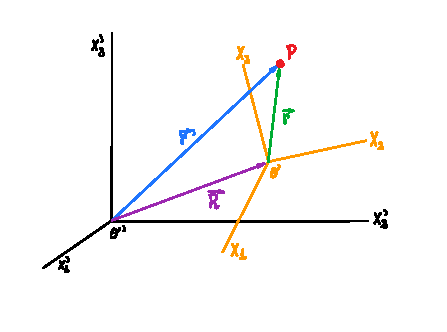
\includegraphics[width=6cm]{noinercial.pdf}
            \caption{Un sistema de referencia \textcolor{blue}{inercial ${\mathcal{O}}'$}  y uno \textcolor{orange}{no inercial $\mathcal{O}$} desde los que se estudia una partícula $P$.}
            \label{fig: noinercial}
        \end{figure}
    \end{marginfigure}

	Antes de comenzar, se va a establecer la notación presente en \Figref{fig: noinercial}, entonces:

	\begin{itemize}
		\item ${\mathcal{O}}'$ : Es el origen del marco de referencia inercial.
		\item $\mathcal{O}$ : Origen del marco de referencia no inercial, con aceleración traslacional y rotación.
		\item $\vec{{r}'}$ : Es el radio vector con origen en ${\mathcal{O}}'$ que da la posición del punto $P$ respecto a dicho origen.
		\item $\vec{R}$ : Es el radio vector con origen en ${\mathcal{O}}'$ que une los marcos de referencia  \textcolor{blue}{inercial ${\mathcal{O}}'$} y \textcolor{orange}{no inercial $\mathcal{O}$}.
		\item $\vec{r}$ :  Radio vector con el origen en $\mathcal{O}$ que da la posición el punto $P$ respecto a dicho origen.
		\item $\vec{omega}$ : Es la velocidad angular con que rota el marco de referencia  \textcolor{orange}{no inercial $\mathcal{O}$}.
	\end{itemize}

	Hecho esto, el objetivo del siguiente desarrollo es deducir la relación diferencial para la derivada temporal de un vector arbitrario (Por ejemplo, el vector posición) entre vectores con origen inercial y vectores con origen no inercial.

	Ahora, por propiedades vectoriales se sabe:

	\begin{equation}
		\vec{{r}'} = \vec{R} + \vec{r}
		\label{eq: posiciondosmarcos}
	\end{equation}

	Suponga que todos estos vectores son medidos desde el marco de referencia \mn{Para referirse de ahora en adelante al marco de referencia desde el que es medido un vector se usará: \begin{itemize} \item \textbf{fijo :} Al medir desde el marco inercial. \\ \item \textbf{rotacional :} al medir desde el marco de referencia no inercial sin importar la naturaleza de la no inercialidad. \\ \end{itemize} } \textcolor{blue}{inercial ${\mathcal{O}}'$} y se aplica la derivada temporal:

	\begin{equation}
		\left( \frac{d \vec{{r}'}}{dt} \right)_{fijo} = \left( \frac{d \vec{R}}{dt} \right)_{fijo} + \left( \frac{d \vec{r}}{dt} \right)_{fijo}
		\label{eq: velocidaddosmarcos}
	\end{equation} 

	Aquí la pregunta, ¿qué pasa si el observador se encuentra en el marco no inercial y desde este se desea realizar los análisis? Hay que obtener una relación que permita lo siguiente:

	\begin{equation*}
		\left( \frac{d \vec{r}}{dt} \right)_{fijo} \leftrightarrow \left( \frac{d \vec{r}}{dt} \right)_{rotacional}
	\end{equation*}

	Entonces, desarrollando la expresión del vector $\vec{r}_{rotacional}$ y derivada temporal (Desde el marco no inercial \mn{Para este tema es fundamental entender en que lugar se encuentra el observador, donde está el origen desde el que se mide. Además, es preciso tener claro las coordenadas que se usan en todo momento.}):

	\begin{align*}
		\vec{r}_{rotacional} &= \sum_{i=1}^{3} r_{i}\hat{e}_{i} \\
		\left( \frac{d \vec{r}}{dt} \right)_{rotacional} &= \sum_{i=1}^{3} \frac{d r_{i}}{dt} \hat{e}_{i}
	\end{align*}

	Ahora la velocidad desde una perspectiva inercial \mn{Aquí va a ser importante recordar \Eqref{eq: vwrelation}, que se puede reescribir de la siguiente forma para aplicarla al caso actual de estudio: \\ \begin{equation*} \left( \frac{d \vec{r}}{dt} \right)_{fijo} =  \vec{\omega} \times \vec{r} \end{equation*} }:

	\begin{align*}
		\left( \frac{d \vec{r}}{dt} \right)_{fijo} &=  \sum_{i=1}^{3} \frac{d r_{i}}{dt} \hat{e}_{i} + \sum_{i=1}^{3} r_{i} \left( \frac{d \hat{e}_{i}}{dt}\right)_{fijo} \\ 
		&= \underbrace{\sum_{i=1}^{3} \frac{d r_{i}}{dt} \hat{e}_{i}}_{\left( \frac{d \vec{r}}{dt} \right)_{rotacional}} + \sum_{i=1}^{3} r_{i} \left(\vec{\omega} \times \hat{e}_{i} \right) \\
		&=  \left( \frac{d \vec{r}}{dt} \right)_{rotacional} + \vec{\omega} \times \sum_{i=1}^{3} r_{i} \hat{e}_{i} \\ 
		&= \left( \frac{d \vec{r}}{dt} \right)_{rotacional} + \vec{\omega} \times \vec{r}
	\end{align*}

	Finalmente se obtuvo la relación de las derivadas temporales entre los sistemas de referencia para el caso de la posición de la partícula $P$:

	\begin{equation}
		\left( \frac{d \vec{r}}{dt} \right)_{fijo} = \left( \frac{d \vec{r}}{dt} \right)_{rotacional} + \vec{\omega} \times \vec{r}
		\label{eq: inertialnoinertialr}
	\end{equation}

	De forma general, dicha relación se puede escribir para cualquier vector:

	\begin{equation}
		\left( \frac{d \vec{G}}{dt} \right)_{fijo} = \left( \frac{d \vec{G}}{dt} \right)_{rotacional} + \vec{\omega} \times \vec{G}
		\label{eq: inertialnoinertialG}
	\end{equation}

	Continuando con la \Eqref{eq: velocidaddosmarcos}, esta expresión se puede reescribir utilizando la \Eqref{eq: inertialnoinertialr}:

	\begin{align*}
		\left( \frac{d \vec{{r}'}}{dt} \right)_{fijo} & = \left( \frac{d \vec{R}}{dt} \right)_{fijo} + \left( \frac{d \vec{r}}{dt} \right)_{fijo} \\ 
		& = \left( \frac{d \vec{R}}{dt} \right)_{fijo} + \left( \frac{d \vec{r}}{dt} \right)_{rotacional} + \vec{\omega} \times \vec{r} \\ 
		& = \dot{\vec{R}}_{f} + \dot{ \vec{r}}_{r} + \vec{\omega} \times \vec{r} \\ 
	\end{align*}

	\begin{definition}[\textbf{Relación entre las velocidades inerciales y no inerciales}]
		\begin{equation}
			\dot{ \vec{{r}'}}_{f} = \dot{\vec{R}}_{f} + \dot{ \vec{r}}_{r} + \vec{\omega} \times \vec{r}
			\label{eq: vinirelation}
		\end{equation}
	\end{definition}


	Derivando la \Eqref{eq: vinirelation} con respecto al tiempo, se llegará a la relación de la aceleración entre los marcos de referencia.

	\begin{align*}
		\left(\frac{d \dot{ \vec{{r}'}}_{f} }{dt}\right)_{f} &= \left(\frac{d  \dot{\vec{R}}_{f} }{dt}\right)_{f} + \left(\frac{d  \dot{ \vec{r}}_{r}}{dt}\right)_{f} + \left(\frac{d  }{dt}\right)_{f} \left( \vec{\omega} \times \vec{r} \right) \\ 
		& = \ddot{\vec{R}}_{f} + \ddot{ \vec{r}}_{r} + \vec{\omega} \times \dot{ \vec{r}}_{r} + \dot{\vec{\omega}} \times \vec{r} + \vec{\omega} \times \dot{\vec{r}}_{f} \\
		& = \ddot{\vec{R}}_{f} + \ddot{ \vec{r}}_{r} + \vec{\omega} \times \dot{ \vec{r}}_{r} + \dot{\vec{\omega}} \times \vec{r} + \vec{\omega} \times \left(\dot{\vec{r}}_{r} + \vec{\omega} \times \vec{r} \right) \\ 
		& = \ddot{\vec{R}}_{f} + \ddot{ \vec{r}}_{r} + \dot{\vec{\omega}} \times \vec{r}  + 2\vec{\omega} \times \dot{ \vec{r}}_{r} + \vec{\omega} \times \left( \vec{\omega} \times \vec{r}  \right)
	\end{align*}

	\begin{definition}[\textbf{Relación entre las aceleraciones inerciales y no inerciales}]
		\begin{equation}
			\ddot{ \vec{{r}'}}_{f}  = \ddot{\vec{R}}_{f} + \ddot{ \vec{r}}_{r} + \dot{\vec{\omega}} \times \vec{r}  + 2\vec{\omega} \times \dot{ \vec{r}}_{r} + \vec{\omega} \times \left( \vec{\omega} \times \vec{r}  \right)
			\label{eq: ainirelation}
		\end{equation}
	\end{definition}

	\subsection{Segunda Ley de Newton para Sistemas No Inerciales}

	A continuación se va a establecer la forma general de la Segunda Ley de Newton y de este modo extender los casos de análisis de este formalismo. A partiendo de la \Eqref{eq: NSecondlawmcons} y posteriormente haciendo uso de la \Eqref{eq: ainirelation}:

	\begin{align*}
		\sum \vec{F} &= m \ddot{\vec{{r}'}}_{f} \\
		& = m \left[ \ddot{\vec{R}}_{f} + \ddot{ \vec{r}}_{r} + \dot{\vec{\omega}} \times \vec{r}  + 2\vec{\omega} \times \dot{ \vec{r}}_{r} + \vec{\omega} \times \left( \vec{\omega} \times \vec{r}  \right) \right] \\ 
		& = m\ddot{\vec{R}}_{f} + m\ddot{ \vec{r}}_{r} + m \dot{\vec{\omega}} \times \vec{r} + 2m \vec{\omega} \times \dot{ \vec{r}}_{r} + m \vec{\omega} \times \left( \vec{\omega} \times \vec{r}  \right) \\ 
		\Rightarrow \sum \vec{F} & - m\ddot{\vec{R}}_{f} -  m \dot{\vec{\omega}} \times \vec{r} - 2m \vec{\omega} \times \dot{ \vec{r}}_{r} - m \vec{\omega} \times \left( \vec{\omega} \times \vec{r}  \right) = m\ddot{ \vec{r}}_{r}
	\end{align*}

	\begin{definition}[\textbf{Segunda Ley de Newton No Inercial}]
		\begin{equation}
			\underbrace{\sum \vec{F}}_{\textup{Fuerzas reales}} - m\ddot{\vec{R}}_{f} -  m \dot{\vec{\omega}} \times \vec{r} \underbrace{- 2m \vec{\omega} \times \dot{ \vec{r}}_{r}}_{\textup{Fuerza de Coriolis}}  \overbrace{- m \vec{\omega} \times \left( \vec{\omega} \times \vec{r}  \right)}^{\textup{Fuerza Centrífuga}} = m\ddot{ \vec{r}}_{r}
			\label{eq: NSecondlawnoinertial}
		\end{equation}
	\end{definition}
	
	Es preciso introducir el concepto de \textbf{fuerzas ficticias}, estas son aquellas ``fuerzas'' que resultan ser introducidas en la Segunda Ley de Newton para generalizar la expresión original (\Eqref{eq: NSecondlawmcons}) de modo que sea capaz de analizar desde marcos de referencia no inerciales. Es decir, estas no son fuerzas o interacciones reales con el entorno; son más bien un artificio que permite ampliar el alcance de la Segunda Ley de Newton.

	\subsection{Problemas resueltos}
	\includepdf[pages={164-182},templatesize = {8 in}{8.5 in} ]{AMeca.pdf}

\end{document}